\documentclass{beamer}
    \usetheme{Boadilla}
\usepackage{polyglossia}
    \setmainlanguage{english}
\usepackage{fontspec}
    \setsansfont{Linux Biolinum O}
\usepackage{graphicx}
\usepackage{xcolor} \usepackage{rotating}
\usepackage{listings}
    \lstset{language=bash,
	basicstyle=\footnotesize\ttfamily\tiny,
	breaklines=true,
	framextopmargin=50pt,
	frame=bottomline,
	backgroundcolor=\color{white!86!black},
	commentstyle=\color{blue},
	keywordstyle=\color{red},
	stringstyle=\color{orange!80!black}}
\usepackage{amsmath}
\usepackage{amssymb}
\usepackage{siunitx}
\usepackage{booktabs}
\usepackage{float}
\usepackage{tabularx}
\usepackage{caption}
\usepackage{subfig}
\usepackage{tikz}
\usepackage{datenumber}
\setbeamertemplate{itemize items}[circle]
\usepackage{hyperref}
     \hypersetup{
     colorlinks=true,
     linkcolor=black,
     filecolor=magenta}

\title{\texorpdfstring{\color{blue!50!black}\textbf{Status report - Thursday}}{}}
\subtitle{Timeline for Bachelor Studies}
\author{Maurice Donner \and David Schledewitz}
\date{September 10th, 2020}

\begin{document}

\maketitle

\begin{frame}{March}
    \begin{itemize}
	\item Starting to work together with Bogdan and Pascal on the ALPIDE
	    Telescope.
	\item Main Operation of the Telescope
	\item What is a Threshold Scan?
    \end{itemize}
\end{frame}

\begin{frame}{April}
    \begin{itemize}
	\item Plotting first results of threshold scans
	    \begin{figure}[H]
		\centering
		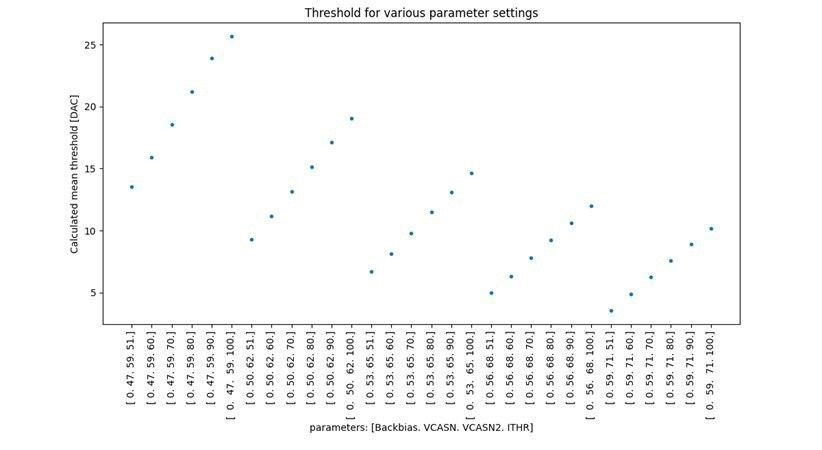
\includegraphics[width=.4\textwidth]{DavidFirst.jpg}
	    \end{figure}
	\item Later that month: Automising the procedure and plotting the first
	    Threshold "Heatmaps"
	    \begin{figure}[H]
		\centering
		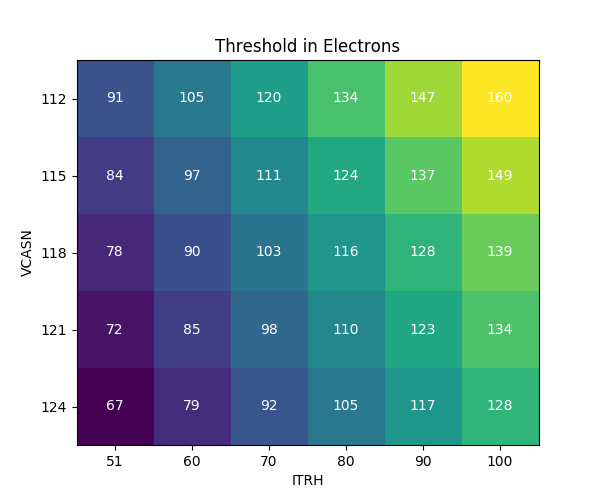
\includegraphics[width=.3\textwidth]{MauriceFirstMaps.png}
	    \end{figure}
    \end{itemize}
\end{frame}

\begin{frame}{April}
    \begin{itemize}
	\item Also finishing the First Google Document
	\item Looking at first Noiseoccupancy Scans
	    \begin{figure}[H]
		\centering
		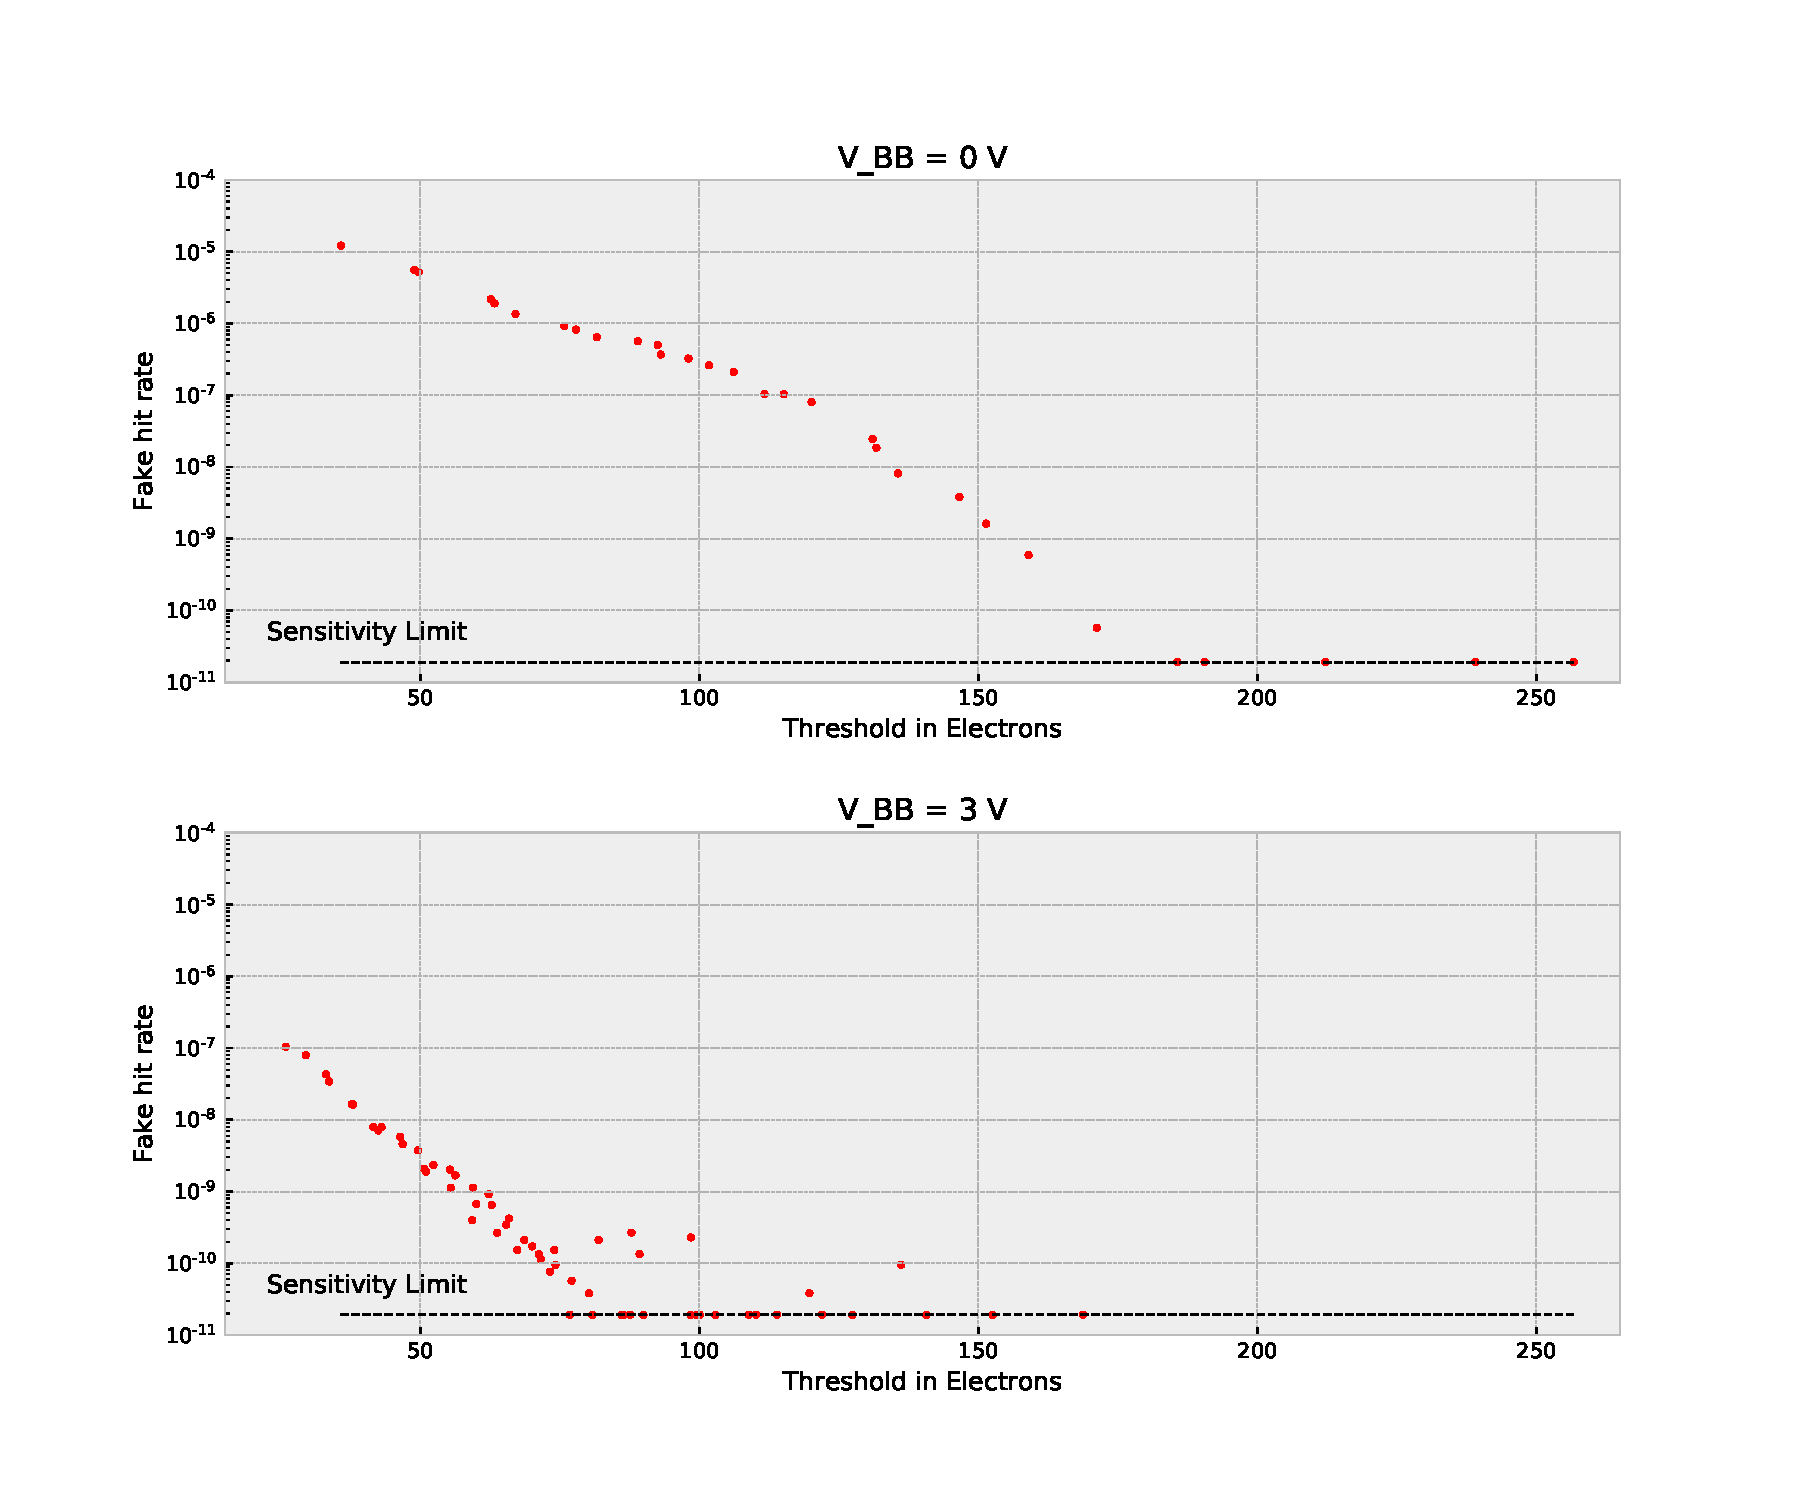
\includegraphics[width=.5\textwidth]{MauriceFirstNoise.pdf}
	    \end{figure}
	\item Deciding to take Cosmic data due to the Health restrictions
	\item Finishing the second Google Document
    \end{itemize}
\end{frame}

\begin{frame}{May}
    \begin{itemize}
	\item Cosmics yield huge filesizes. Starting to work on a program that
	    handles them...
	\item Meanwhile keep taking as much data as possible, and
	    documenting the process in another Google Document
	    \begin{figure}[H]
		\centering
		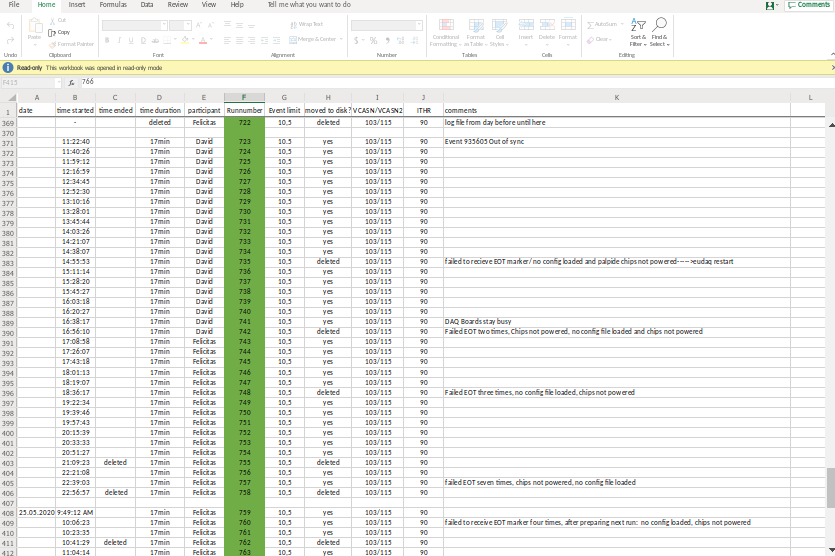
\includegraphics[width=.4\textwidth]{DavidCosmicProgress.png}
	    \end{figure}
    \end{itemize}
\end{frame}
\begin{frame}{May}
    \begin{itemize}
	\item Looking especially at Muon rates, chip effectiveness and
	    making first calculations about angular distributions
	    \begin{figure}[H]
		\centering
		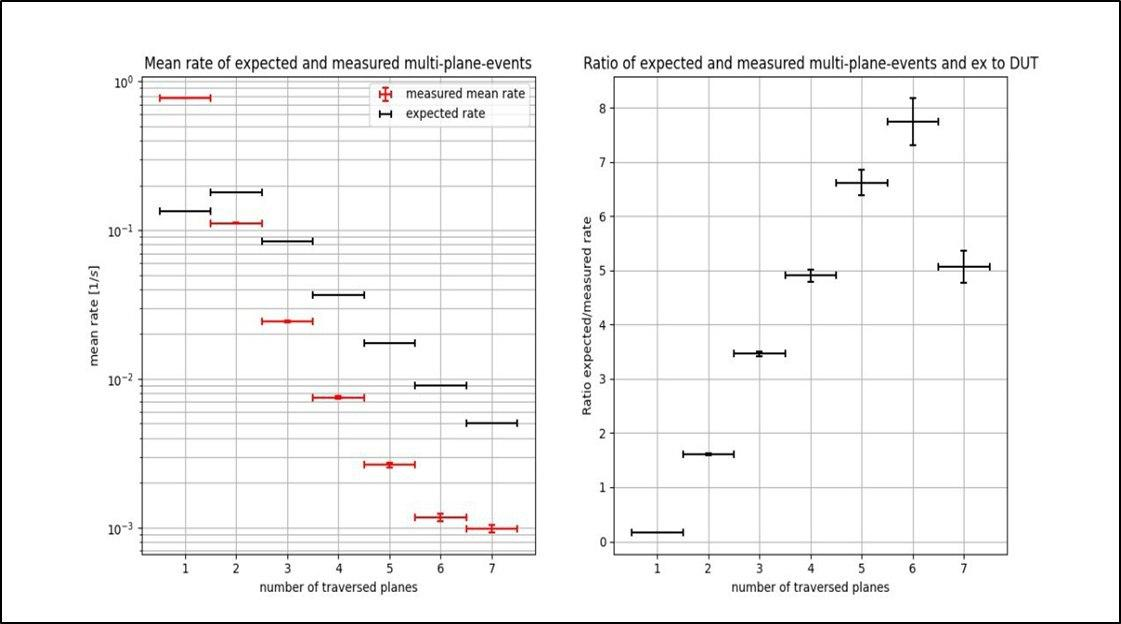
\includegraphics[width=.4\textwidth]{DavidFirstRate.jpg}
		\
		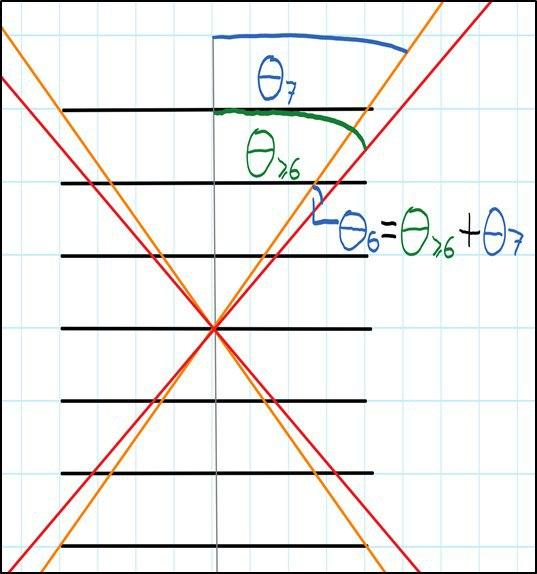
\includegraphics[width=.25\textwidth]{DavidFirstAngle.jpg}
	    \end{figure}
	    \begin{figure}[H]
		\centering
		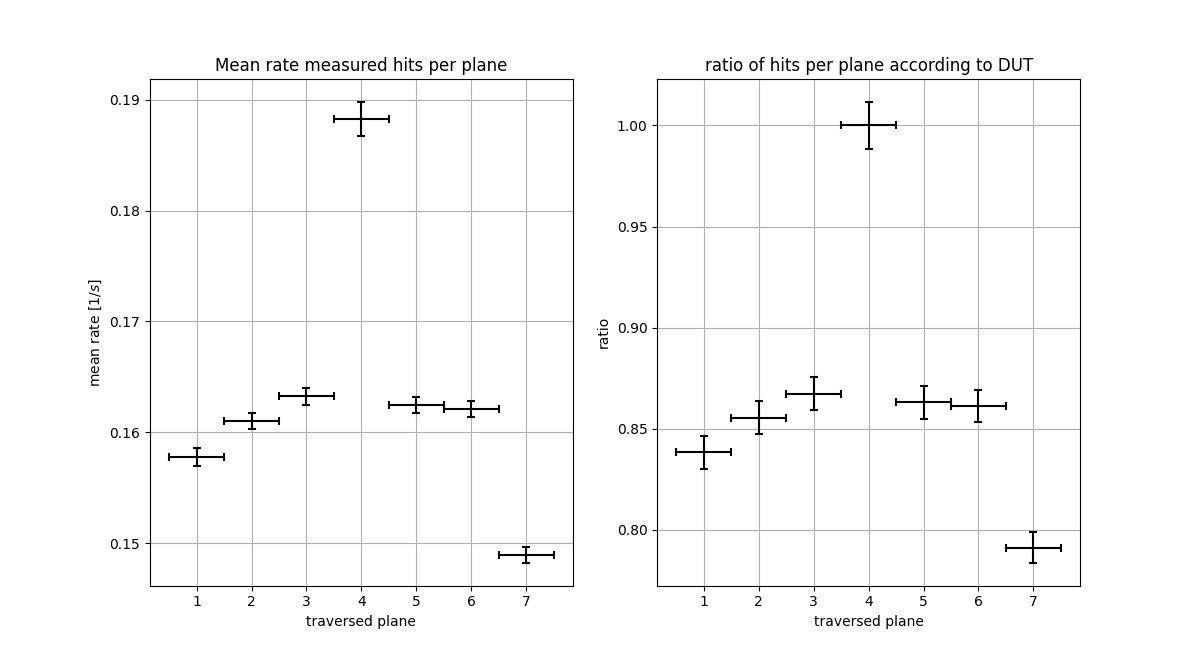
\includegraphics[width=.4\textwidth]{DavidFirstEff.jpg}
	    \end{figure}
    \end{itemize}
\end{frame}

\begin{frame}{June}
    \begin{itemize}
	\item Finishing the compression program, and taking first looks at the
	    cosmic data as a whole
	    \begin{figure}[H]
		\centering
		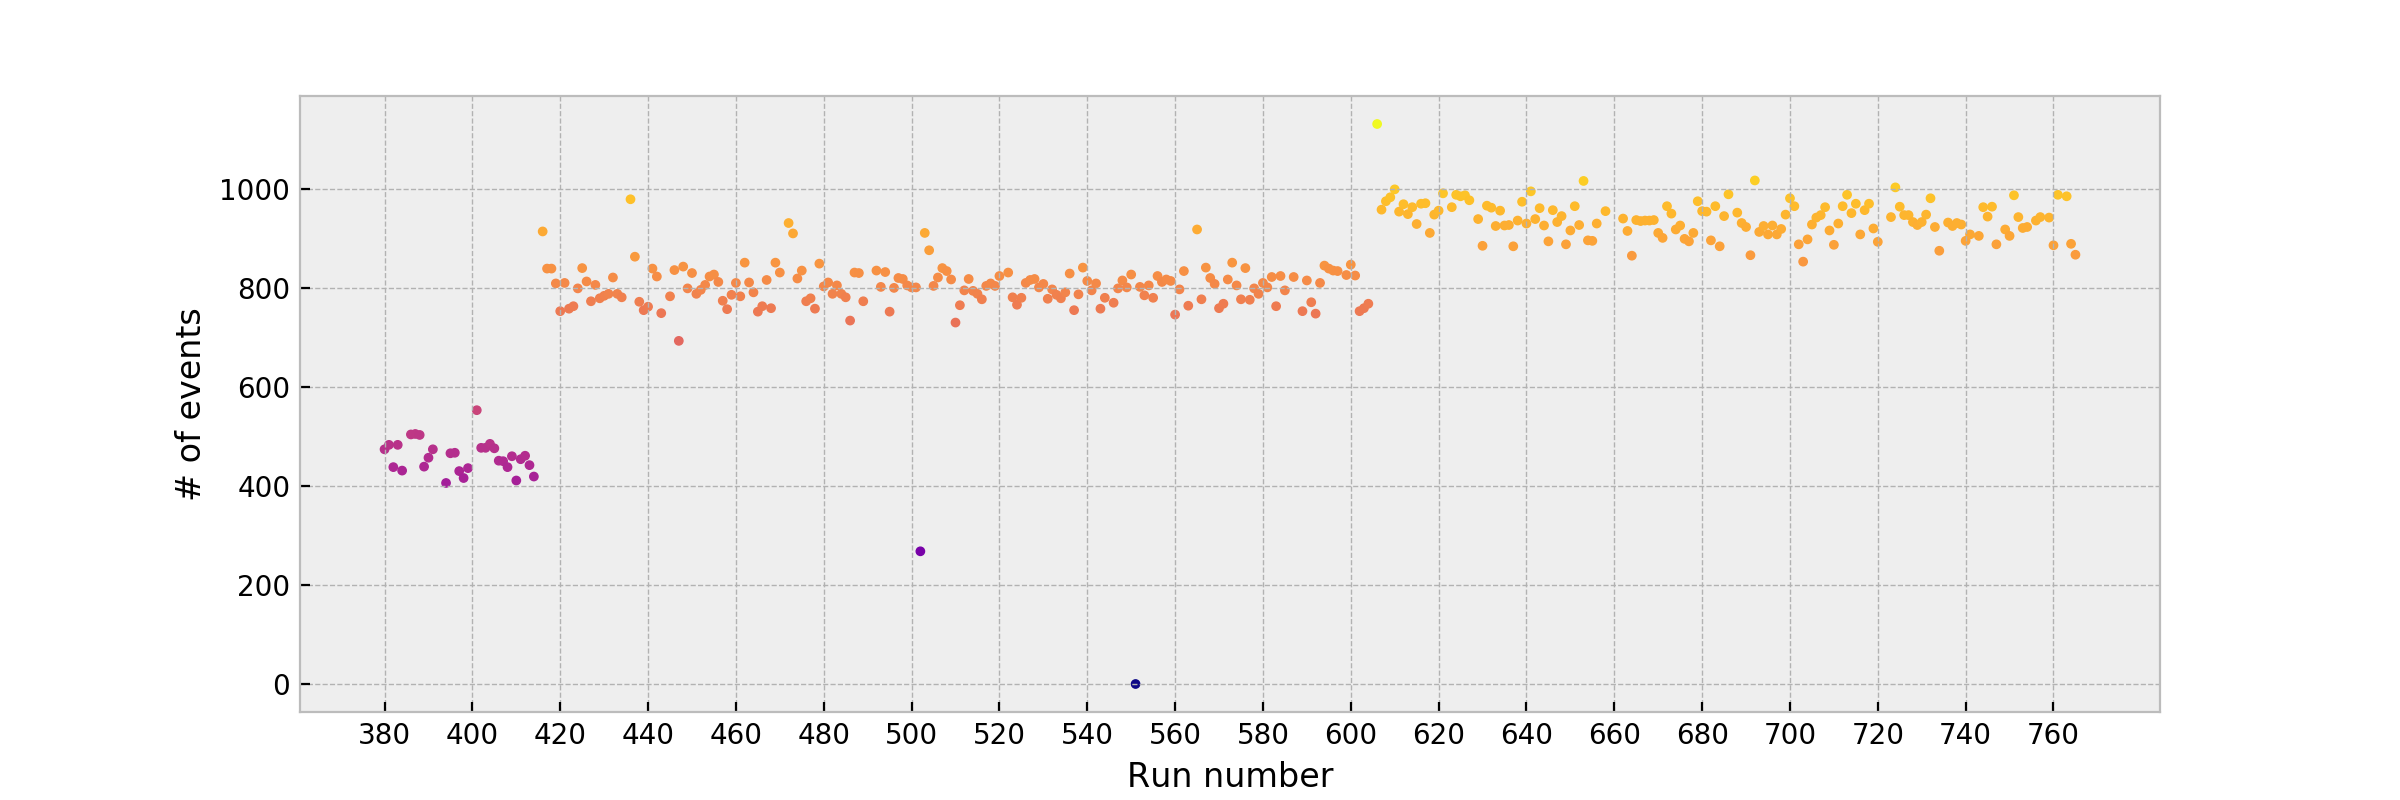
\includegraphics[width=.9\textwidth]{MauriceFirstLookCosmics.png}
	    \end{figure}
	\item Starting to work on a tracking algorithm, since the data per run
	    is too small for corryvreckan
    \end{itemize}
\end{frame}

\begin{frame}{June}
    \begin{itemize}
	\item Fixing muonrate calculations and looking at overestimation
	    \begin{figure}[H]
		\centering
		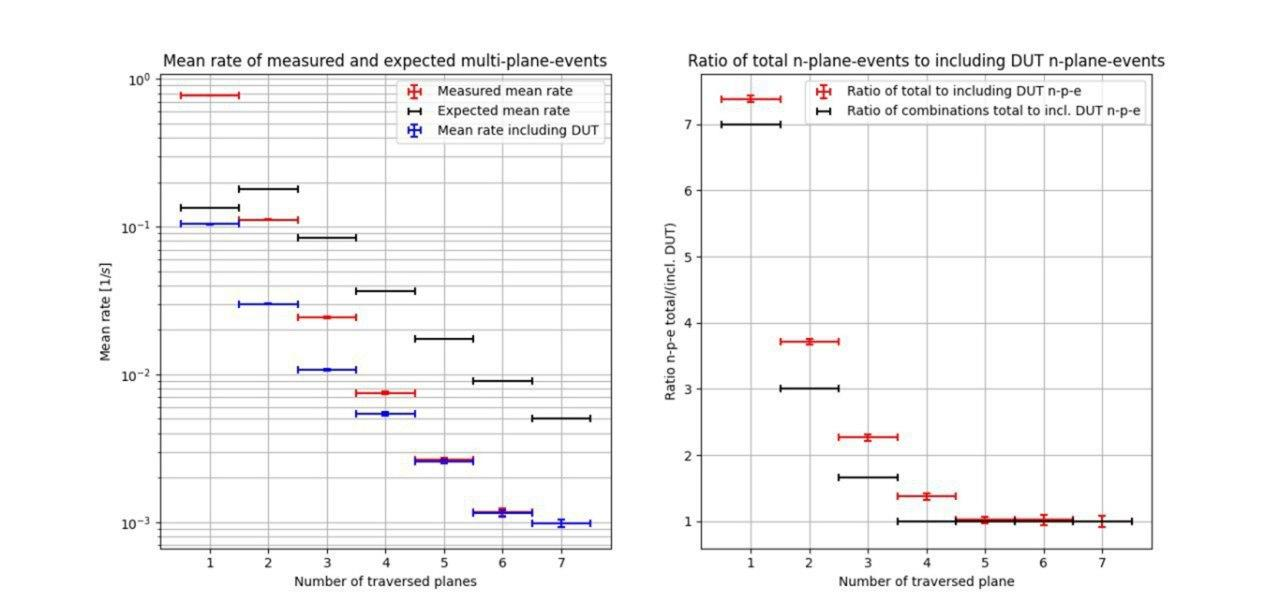
\includegraphics[width=.9\textwidth]{DavidOverestimation.jpg}
	    \end{figure}
    \end{itemize}
\end{frame}

\begin{frame}{July}
    \begin{itemize}
	\item Finishing Event organization and first align attempts
	    (First with Testbeam Data)
	    \begin{figure}[H]
		\centering
		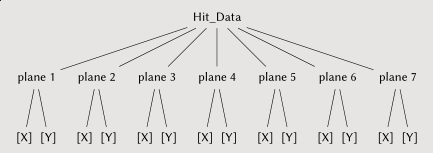
\includegraphics[width=.4\textwidth]{MauriceEventOrg.png}
		\
		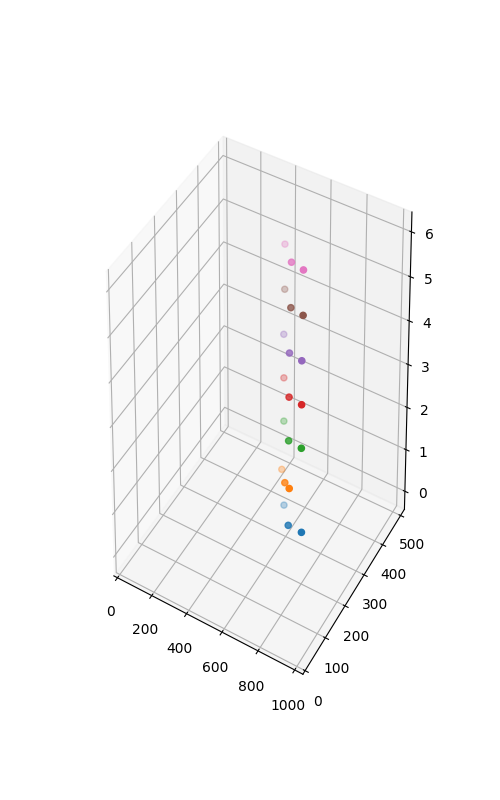
\includegraphics[width=.15\textwidth]{MauriceFirstAlign.png}
	    \end{figure}
	\item Meanwhile visualizing the first Cosmics
	    \begin{figure}[H]
		\centering
		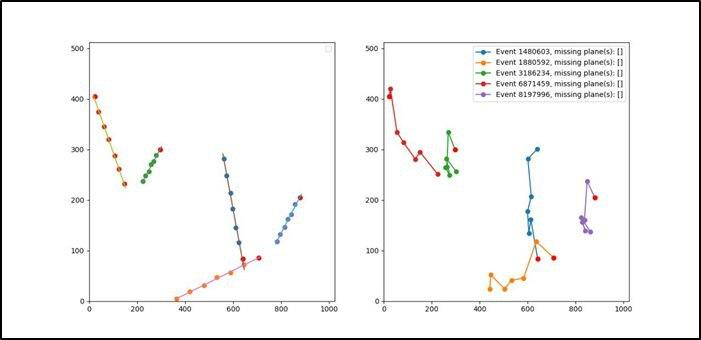
\includegraphics[width=.4\textwidth]{DavidFirstVisual.jpg}
	    \end{figure}
    \end{itemize}
\end{frame}

\begin{frame}{July}
    \begin{itemize}
	    \footnotesize
	\item Finished Tracking algorithm and comparing 
	    alignment to DESY-Testbeam Data
	    \begin{figure}[H]
		\centering
		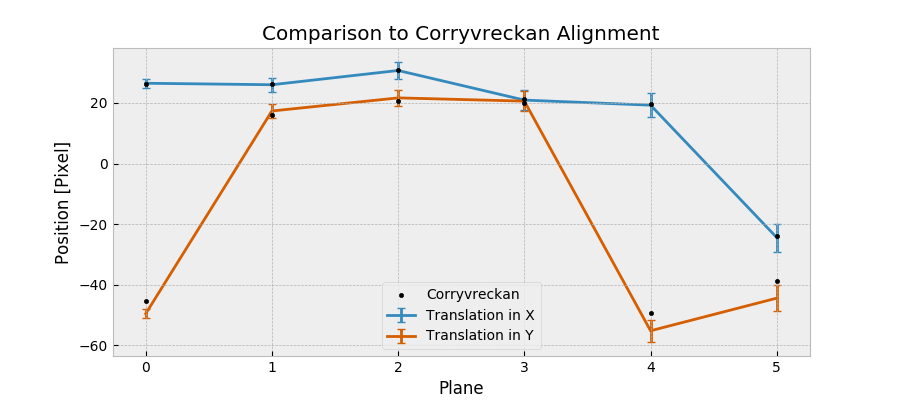
\includegraphics[width=.49\textwidth]{Corry.png}
		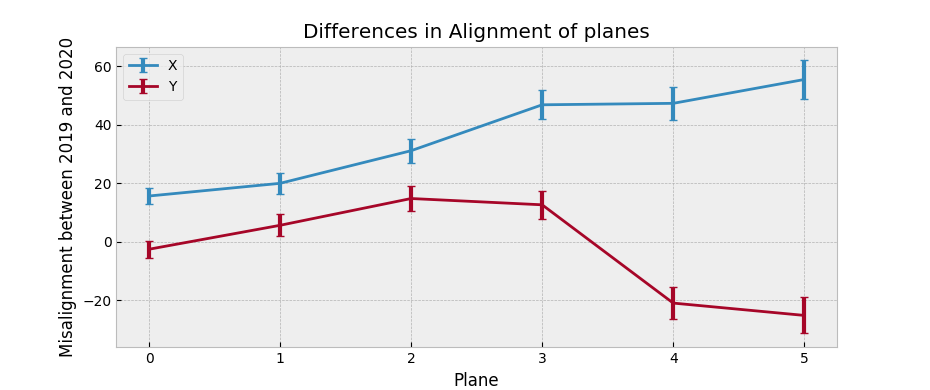
\includegraphics[width=.49\textwidth]{Misalignment.png}
	    \end{figure}
	\item Found out, that transporting the telescope changes the alignment
	    by up to 1.7mm.
	\item Looking at \( \chi^2 \) and identifying further alignment issues
	    \begin{figure}[H]
		\centering
		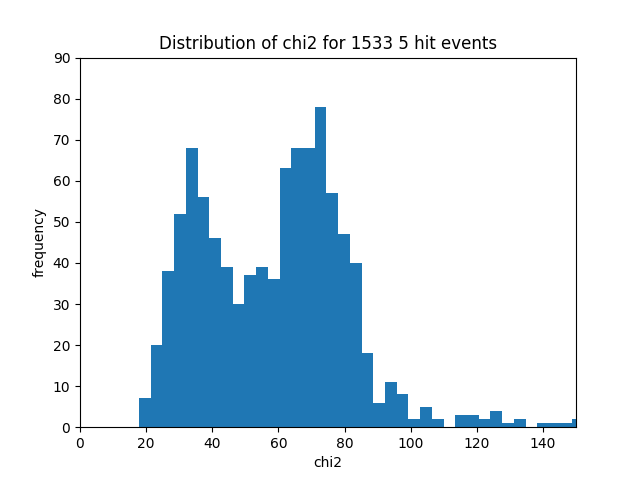
\includegraphics[width=.4\textwidth]{MauriceChi2.png}
		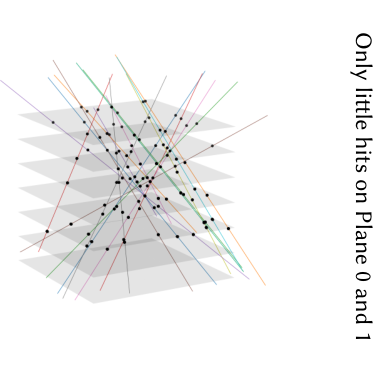
\includegraphics[width=.3\textwidth]{MauriceMisalign.png}
	    \end{figure}
    \end{itemize}
\end{frame}
\end{document}
